\section{Introduction}

Large Language Models (LLMs) now dominate natural language processing (NLP) \citep{devlin2019bert, brown2020language, kaplan2020scaling, ouyang2022training, wei2022emergent, wei2022chain, touvron2023llama, openai2024gpt4technicalreport}, powering chatbots \citep{anthropic2023claude, bai2023qwen, openai2024gpt4technicalreport, deepseekai2025deepseekr1incentivizingreasoningcapability}, search engines \citep{google2023bard, microsoft2023bing}, and programming assistants \citep{copilot, claude_3_7}. These models generate text through \textit{inference}---producing responses to user queries---which imposes significant computational demands on memory and processing resources \citep{garcia2019estimation}. Systems like ChatGPT incur daily inference costs exceeding \$700,000 and contribute to substantial carbon emissions \citep{patel2023peeling, patterson2021carbon}. Efficient inference scheduling can reduce these operational costs and energy consumption \citep{strubell2019energy, desislavov2021compute} by balancing system throughput and response latency \citep{wu2022sustainable}.

To design effective scheduling, we must first understand the LLM inference process. Figure~\ref{fig:intro_example} provides a step-by-step illustration of how a query is processed during inference. The process begins when a user submits a prompt—e.g., ``Is apple a fruit?''—which is then passed through several computational stages. The inference pipeline consists of two main phases:
\begin{itemize}
    \item \textbf{Prefill Phase (stage 0)}: Upon receiving the prompt, the model first tokenizes the input into a sequence of discrete units (e.g., ``Is'', ``apple'', ``a'', ``fruit'', ``?''). These tokens are then embedded and simultaneously processed in a single forward pass to compute the \textit{Key-Value (KV) cache}, which stores intermediate representations (i.e., attention keys and values) for each token. These precomputed values enable efficient reuse during subsequent decoding steps. This phase corresponds to Stage 0 in Figure~\ref{fig:intro_example}, where all prompt tokens are embedded and their KV representations are added to the cache.

    \item \textbf{Decode Phase (stages 1 to $l^\prime$)}: After the prefill phase, the model enters the decode phase, where it generates the output one token at a time. At each stage, the model queries the existing KV cache to compute the next token, appends the new token to the output sequence, and updates the KV cache with its key-value pair. For instance, the model might first generate ``Yes'' (Stage 1), then ``it'' (Stage 2), followed by ``is'' (Stage 3), and finally the ``End of Sequence'' (EOS) token (Stage 4). This progression is depicted in the lower part of Figure~\ref{fig:intro_example}. Each token generation step involves both reading from and writing to the KV cache, resulting in a memory footprint that grows linearly with the length of the generated sequence.
\end{itemize}

Figure~\ref{fig:intro_example} also highlights key performance metrics in LLM inference:
\begin{itemize}
    \item \textbf{Time-To-First-Token (TTFT)} measures the latency from user input to the first generated token.
    \item \textbf{Latency} refers to the total time required to complete the generation of all output tokens.
    \item \textbf{Throughput} captures the average number of tokens generated per unit time.
\end{itemize}

This inference structure, particularly the growing memory requirements and sequential decoding pattern, introduces fundamental constraints on scheduling and batching. Efficient scheduling must account for both prompt heterogeneity and KV cache dynamics to balance latency and resource use.

\begin{figure}
    \centering
    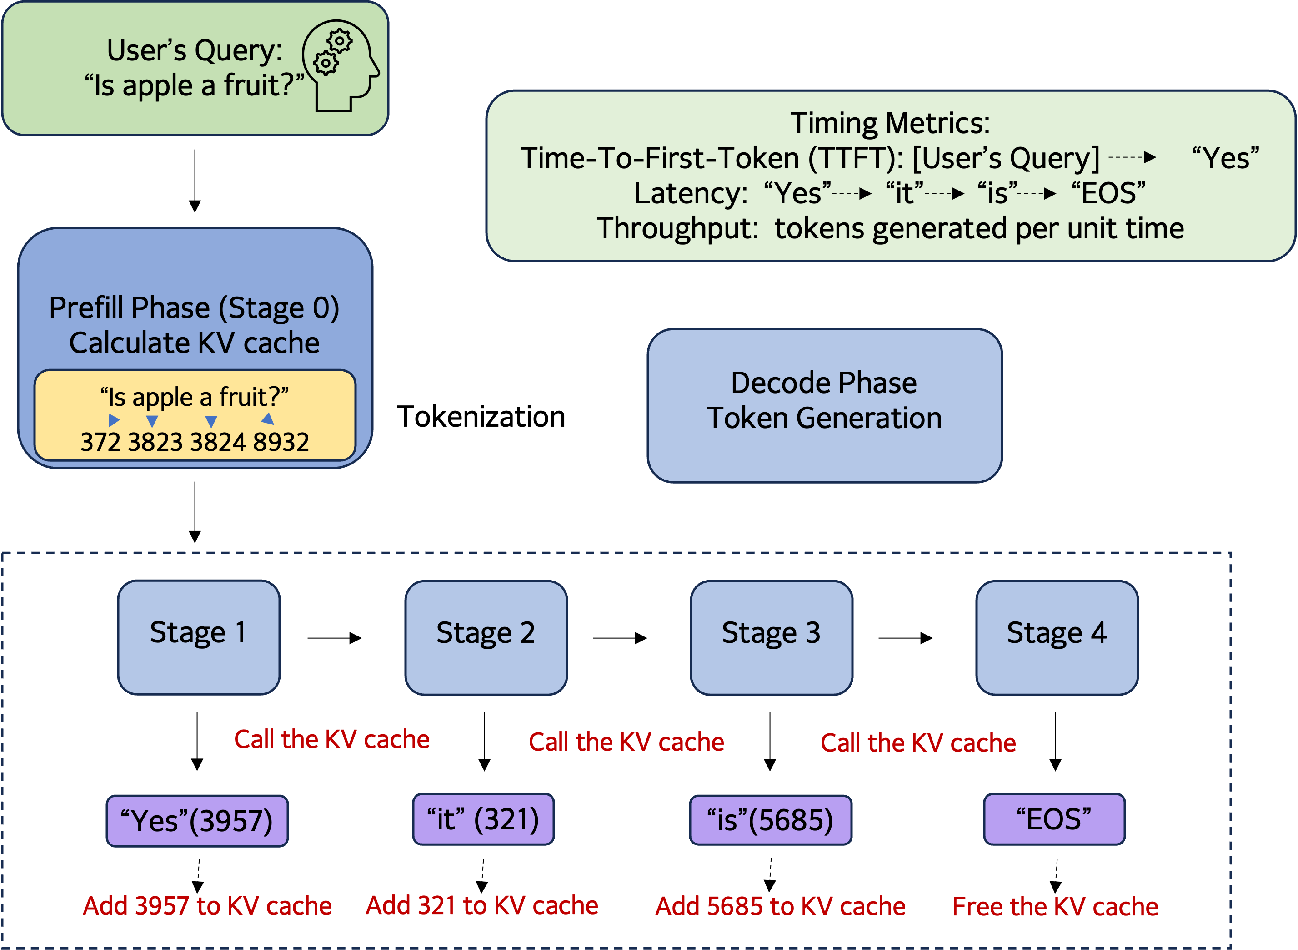
\includegraphics[width=0.6\linewidth]{Experiments_pdf/fig_intro.pdf}
    \caption{An example of LLM inference.}
    \label{fig:intro_example}
\end{figure}

Scheduling LLM inference tasks involves grouping prompts into \textit{batches} processed concurrently on a GPU. Batching improves throughput: processing multiple prompts together amortizes the fixed overhead of each iteration and better uses GPU parallelism. However, this benefit comes with a fundamental tension---larger batches consume more memory through their combined KV caches. The KV cache improves efficiency, as it prevents the model from recalculating attention history for each new token; without it, computational cost would scale quadratically with sequence length. But the KV cache also grows dynamically during decode, making memory footprint unpredictable. This creates a core trade-off: \emph{larger batches increase throughput but consume more memory, risking capacity overflow}.

Memory overflow can occur in several practical scenarios: (i) \emph{bursty arrivals}, where sudden traffic spikes temporarily exceed capacity; (ii) \emph{unknown output lengths}, where prompts generate longer responses than anticipated; and (iii) \emph{multi-tenant environments}, where multiple users compete for GPU memory. The unknown output length problem is particularly challenging: since the scheduler cannot predict how much memory each prompt will eventually consume, it cannot reliably plan batch composition or admission decisions. Traditional scheduling methods such as Shortest Job First (SJF) assume fixed job sizes and known processing times, making them unsuitable when memory demands grow unpredictably \citep{tay2022efficient, kang2024gear, hooper2025kvquant}.

\textbf{The Eviction Challenge.} When the total KV cache exceeds GPU memory capacity, the system must evict some in-progress prompts. Two approaches exist: (i) \emph{swapping} to CPU/SSD, incurring I/O overhead \citep{sheng2023flexgen, aminabadi2022deepspeed}; or (ii) \emph{recomputation}, where the KV cache is discarded and the prompt restarts from prefill \citep{kwon2023efficient}. We focus on recomputation because: (1) it is the default in modern production systems such as vLLM \citep{vllm-v1-2025}; and (2) our goal is to \emph{minimize eviction} through intelligent scheduling, rather than optimizing the eviction mechanism itself \citep{li2025mirage}. Eviction creates a vicious cycle: freeing memory temporarily, but restarted prompts consume resources again, potentially triggering further evictions---users may experience this as error messages (e.g., ``Something went wrong'') or incomplete responses under heavy load.

\emph{Memory sufficiency alone does not guarantee stability}. The key to maximizing throughput is \emph{load balance}---the equilibrium state where arrival and completion rates match. Yet even when total capacity $C$ exceeds the optimal steady-state memory $M^*$ (derived in our fluid analysis), naive policies can push the system away from equilibrium. For instance, first-come-first-served (FCFS) can trigger cascading evictions that reduce throughput by 12--25% even when capacity is theoretically sufficient (Example~\ref{ex:fcfs_cascade}). A slight imbalance causes one prompt type to overflow, triggering evictions; the freed memory then fills with another type, which itself overflows, creating a vicious cycle. Thus, a system that \emph{should} be stable becomes unstable under poor scheduling.

Preventing eviction requires \emph{approaching load balance through controlled admission}. Effective scheduling demands not just sufficient capacity, but maintaining the system near equilibrium by carefully controlling when prompts advance to the next decode stage. This "approaching load balance" principle guides our algorithm design: threshold-based mechanisms hold prompts at decode stage boundaries until memory conditions permit safe continuation, keeping the system close to the balanced fluid dynamics.

Recent system-level optimizations for LLM inference \citep{yu2022orca, kwon2023efficient, agrawal2023sarathi, pope2023efficiently, deepseekai2024deepseekv2strongeconomicalefficient, patel2024splitwise, zhong2024distserve} focus on engineering solutions but lack a rigorous mathematical foundation. In practice, output length predictions are imprecise or costly \citep{fu2025efficient}, and algorithms designed for known output lengths can degenerate significantly when this assumption fails (see Proposition~\ref{prop:unknown_lower_bound}).

\textbf{Our Approach.} We develop a fluid dynamics approximation that provides fundamental insights into LLM inference scheduling. The fluid model reveals the equilibrium state---where prompt arrivals and completions balance---and characterizes the optimal steady-state memory $M^*$ that maximizes throughput. This equilibrium serves as a target: when the stochastic system operates near this balanced state, it achieves high throughput while avoiding eviction. The fluid analysis shows that exploiting memory is key to throughput---larger batches process more prompts per iteration, maximizing GPU utilization.

Guided by these fluid insights, we design threshold-based algorithms that keep the stochastic system close to the fluid equilibrium. The WAIT algorithm demonstrates this for known output lengths: threshold-based admission control at each decode stage prevents the system from drifting away from balance. For unknown output lengths, we introduce Nested WAIT, which classifies prompts \emph{on-the-fly}---short prompts complete early and exit, while longer prompts naturally advance to later segments, all without requiring output length prediction. Both algorithms achieve asymptotic optimality by approaching the fluid equilibrium. 

\subsection{Summary of Contributions}

This work contributes to LLM inference scheduling through the following contributions:
\begin{itemize}
\item \textbf{Memory-Constrained Scheduling Model}: We develop a multi-stage online scheduling model that captures the dynamic growth of KV cache memory during LLM inference, where exceeding capacity triggers costly prompt evictions (Section \ref{sec:model}). Using a fluid dynamics approximation from queueing theory, we characterize the optimal throughput and steady-state memory $M^*$ under perfect scheduling (Section \ref{sec:fluid}).
    \item \textbf{Eviction-Prevention Scheduling Algorithms}: We develop threshold-based algorithms that prevent memory overflow and minimize eviction. The WAIT algorithm (Section \ref{sec:wait}) demonstrates the core insight for known output lengths, while the \textit{Nested WAIT} algorithm (Section \ref{sec:nested_wait}) extends this to unknown output lengths through on-the-fly type classification. Both achieve asymptotic optimality via coupling arguments.
    \item \textbf{Experimental Validation}: We evaluate our algorithms on synthetic and real-world datasets, outperforming benchmarks like vLLM \citep{kwon2023efficient} and Sarathi \citep{agrawal2023sarathi}, which are widely recognized high-performance inference engines, in average throughput using Llama2-7B on a single A100 GPU (Section \ref{sec:experiments}).
\end{itemize}
These contributions bridge operations research and machine learning, providing a theoretical framework for memory-constrained LLM inference scheduling that explicitly addresses the eviction problem. Memory-constrained LLM inference initially appears as a complex multi-stage stochastic system with feedback through eviction. Our threshold mechanism transforms this into a tractable problem amenable to queueing analysis by decoupling the interactions between prompt types. Our framework is directly applicable to Prefill-Decode Disaggregated systems such as DistServe \citep{zhong2024distserve} and Splitwise \citep{patel2024splitwise}, where the decode server handles only decode operations, making the linear iteration time model (Section~\ref{sec:model}) exact.
% The paper is structured to elucidate these advancements:
% \begin{itemize}
%     \item \textbf{Section 2} delineates the scheduling problem and its objectives.
%     \item \textbf{Section 3} details the fluid model for throughput optimization.
%     \item \textbf{Section 4} presents the booking-limit algorithm for known prompt types.
%     \item \textbf{Section 5} extends this to a nested algorithm for unknown output lengths.
%     \item \textbf{Section 6} reports numerical findings validating our approach.
%     \item \textbf{Section 7} concludes with implications and future research avenues.
% \end{itemize}

\subsection{Other Related Work}

\paragraph*{Online Scheduling Problem and Queueing System.} 
Classical online scheduling problems focus on optimally assigning jobs that arrive sequentially, each with varying completion times. In settings with stochastic arrivals, foundational studies such as \cite{devanur2009adwords,vee2010optimal,cole2014sample,balkanski2016power,lattanzi2020online} have developed algorithms that learn arrival patterns or distributions to refine scheduling strategies over time. Beyond individual job processing, works like \cite{im2013online,lucier2013efficient,liu2015online,li2020online} have explored simultaneous batching and scheduling, grouping similar jobs to enhance efficiency. Within queueing theory, fluid models serve as first-order approximations of stochastic systems, enabling near-optimal control strategies \cite{mandelbaum1998strong,maglaras2000discrete,bauerle2002optimal,liu2011network}, while asymptotic analysis offers insights into long-term system behavior. However, these traditional approaches do not account for key features of LLM inference that complicate asymptotic analysis: (i) iteration time varies with batch composition and current KV cache sizes, precluding fixed service time assumptions; (ii) memory footprint grows dynamically during decode as new tokens are generated; (iii) out-of-memory (OOM) events trigger prompt eviction, creating feedback loops---classical stability and limit theorems assume jobs complete once started, whereas eviction invalidates standard drift arguments.

\paragraph*{LLM Inference.} 
Theoretical frameworks for analyzing Large Language Model (LLM) inference are scarce, despite their widespread use. Unlike traditional scheduling, LLM inference involves stochastic arrivals, dynamic memory constraints, and multi-phase processing, complicating analytical efforts. System-level works like \cite{patel2023peeling} (``Splitwise") and \cite{zhong2024distserve} (``DistServe") split inference into prompt handling and pipeline execution, while scheduling methods such as \cite{yu2022orca}, \cite{agrawal2023sarathi}, and \cite{agrawal2024taming} use batching to boost throughput—similar to our approach. Other optimizations include \cite{deepseekai2024deepseekv2strongeconomicalefficient} with multi-head latent attention and low-rank KV compression, and \cite{fu2025efficient} with Kendall's Tau for prioritizing prompts by predicted output lengths. These works focus on engineering efficiency and system design. 
% More recently, \cite{jaillet2025onlineschedulingllminference} offers a notably theoretical framework, modeling LLM inference as an online scheduling problem and analyzing an adapted shortest-job-first algorithm with near-optimal regret—yet it assumes known output lengths at arrival, a condition rarely met in practice due to their unpredictability and estimation costs (for example, another neural network may be used at the input side). 
From an operations research perspective, several recent works analyze LLM inference scheduling from an online algorithms viewpoint, focusing on competitive ratio and regret bounds. \cite{jaillet2025onlineschedulingllminference} develops an online scheduling algorithm with near-optimal regret guarantees for settings with known output lengths. \cite{wang2025llm} studies optimization with variable prefill and decode lengths in pipeline parallelism settings. \cite{chen2025adaptively} addresses robust optimization under prediction uncertainty, considering adversarial scenarios. These works provide worst-case performance guarantees that complement our fluid-based approach, which targets asymptotic optimality in throughput. In parallel, \cite{li2025throughput} proposes a stochastic processing model with general batch processing time—including piecewise linear iteration time that captures transitions between compute-bound and memory-bound regimes—demonstrating that work-conserving algorithms achieve optimal throughput. Regarding output length uncertainty, \cite{jaillet2025onlineschedulingllminference} and \cite{wang2025llm} assume known output lengths at arrival, \cite{chen2025adaptively} considers adversarial unknown lengths, while our Nested WAIT algorithm addresses stochastic unknown output lengths through on-the-fly classification. Their frameworks employ modeling abstractions tailored to competitive ratio analysis, while our model explicitly captures memory-dependent iteration time (Equation~\eqref{eq:time_consump}) to analyze the throughput-memory trade-off and eviction prevention mechanisms central to our contribution.


\subsection{Notations}
For integer $n\ge 1,$ we denote $[n]=\{1,2,\dots,n\}$ as the set of integers from $1$ to $n$. For $x\in\real$, denote $\lceil x\rceil$ as the smallest integer not smaller than $x$ and $\lfloor x\rfloor$ as the largest integer not greater than $x$. Denote $x_+=\max\{x, 0\}$. For set $S$, denote $|S|$ as its cardinality. For two functions $f(T)$ and $g(T)$, we use $f(T)=O(g(T))$ if there exists constant $c_1>0$ such that $f(T)\le c_1g(T)$ as $T\to+\infty$ and $f(T)=\Omega(g(T))$ if there exists constant $c_2>0$ such that $f(T)\ge c_2g(T)$ as $T\to +\infty$. 